%12章

\chapter{牛顿运动定律}
\label{ch:Newton's Law of Motion}
在这一章中,将系统性地学习牛爵爷所带来的船新版本的物理经典力学的支柱内容。

\section*{学习目标}
\begin{todolist}
	\item 理解牛顿第一定律
	\item 理解牛顿第二定律
	\item 理解牛顿第三定律
	\item 求算竖直方向的运动
	\item 求算斜坡方向的运动
	\item 求算涉及连接的物体的运动和力
\end{todolist}
\clearpage

\section{牛顿运动学三大定律}
这三大定律是物理学开始正式成为一门严谨的自然科学的第一枪。
\subsection*{牛顿第一定律}
实际上,在\ref{sec:Conditions for equilibrium}中,我们就已经见到了牛顿第一定律了,只不过还不够完整。当时强调的平衡状态是静止,但是还有一种平衡状态是匀速直线运动。因此完整版的牛顿第一定律是:
\begin{theorem}
An object will remain at rest or in a state of uniform motion unless it is acted on by a resultant force.
\end{theorem}
通俗易懂来讲,就是物体如果受力平衡,那么物体要么保持静止的状态,要么保持匀速直线运动。因此这两个状态就称之为平衡状态,将受力和运动联系在一起。在考试中看到at rest,uniform motion等字眼一定要和Equilibrium联系到一起

\subsection*{牛顿第二定律}
牛顿第二定律可以认为是三大定律当中最为重要的定律,也被称之为加速度定律。其陈述如下:
\begin{theorem}
The resultant force acting on an object is directly proportional to the rate of change of the linear momentum of that object. The resultant force and the change in momentum are in the same direction.
\end{theorem}

而这里的rate of change of momentum其实就来源于之前我们所研究的内容,换成更简单的可理解的概念,其实就是力。因此牛顿第二定律的等效描述:
\begin{corollary}
一个物体的加速度与作用在该物体上的合外力成正比,与该物体的质量成反比。
\end{corollary}

写成公式则是:
\[
	F=ma \quad  \text{or} \quad a=\frac{F}{m}
\]
该定律直观性地告诉人们,作用在物体上的力能够使物体产生加速度,从而改变物体运动状态,因此动力学和运动学其实是不分家的。都是经典力学的重要组成部分。

\subsection*{牛顿第三定律}
牛顿第三定律也被称之为作用力与反作用力定律,并不是分析一个物体,而是两个物体之间的互相作用力。其表述如下:
\begin{theorem}
When two bodies interact, the forces they exert on each other are equal and opposite.
\end{theorem}
提炼核心信息为:大小相等,方向相反,作用在两个物体上。这个定律都已经有点哲学的味道了。
\clearpage

\section{重力与自由落体}
之前讲过重力的大小与质量成正比,当中用了$W=mg$这样的公式,$g$就是重力和质量的比值,因此当时说$g$的单位是\si{\N\per\kg}。但那并不是$g$的最常见的意义。
考虑一个物体在\emph{仅有}重力的作用的时候,结合一下牛顿第二定律,就可以知道,这个物体必定是加速下落的。而且轨迹一定为直线。那么现在这个下落的加速度的求算,就可以运用牛顿第二定律进行求算:
\[
	a=\frac{W}{m}=\frac{mg}{m}=g
\]
因此,$g$的另一重身份,就显露出来的,它是一个加速度!由于是因为重力导致的,而这也是砸在牛顿的苹果\footnote{苹果的说法是晚年的时候,牛顿的侄女宣扬的。并没有明确史料记载,很有可能是出于牛顿的教徒身份而进行的宣传}为什么会下落的原因因此称之为\gls{accdueg} 此时$g$的单位就变成了$10$ \si{\m\per\square\s}\footnote{仅在A-Level数学部分的$g=10$,$g$更精确的数值是$9.81$,再精确一点的说法是地球上海拔,经纬度的不同的地方,$g$值都略有微小变化}。

\subsection*{自由落体}
\label{subse:Free Fall}
在之前的公式中,不难发现,这个加速度和物体的质量没有关系,也就是说,理论上,任何物体都会以同样的重力加速度向下运动。因此无论在那个时刻都有一样的运动状态。最终会同时落地。而这样的推导在伽利略的比萨斜塔实验\footnote{伽利略很有可能没有做过比萨斜塔实验,是其弟子宣传。伽利略的证明方法是思想实验,推出矛盾}之前都一致保持着亚里士多德的``重的物体先落地''的错误观点。但是有没有发现,只要定量研究的方法确定出来,古希腊的先哲们的观点很多都会毫无根据,不够严谨。
\begin{figure}[H]
\centering
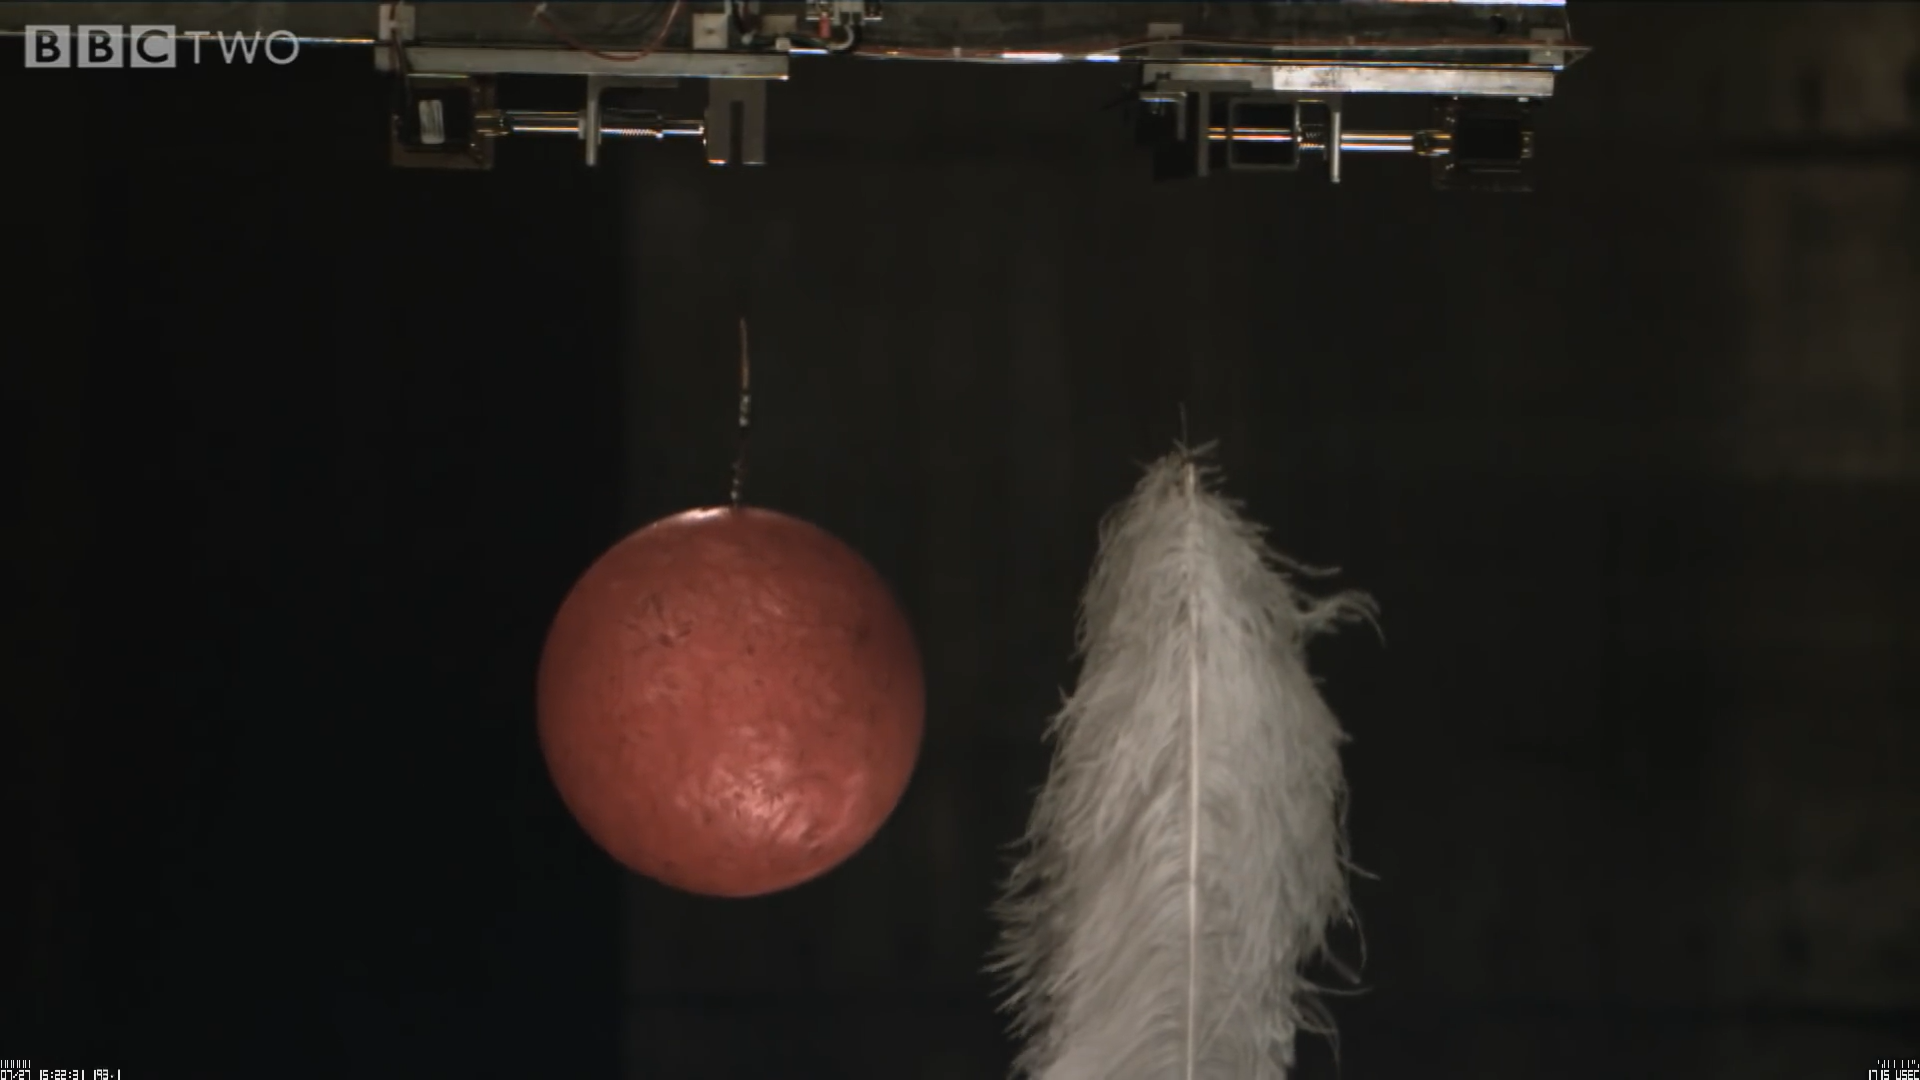
\includegraphics[width=0.8\textwidth]{feather}
\caption{保龄球和羽毛在慢动作下都是具有共同的速度}
\end{figure}

因此结合之前的匀加速直线运动的公式,对于一个\gls{freefall}的运动,初速度$u=0$,加速度$a=g$,自由落体运动的$v-t$图如下:
\begin{figure}[H]
\centering
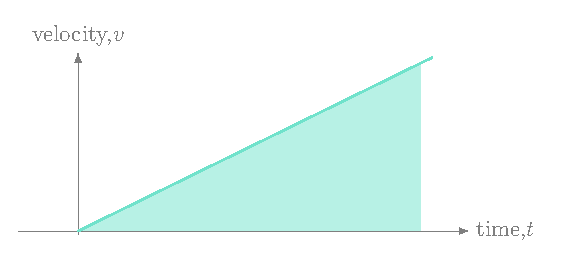
\includegraphics[width=0.8\textwidth]{freefall}
\caption{自由落体的$v-t$图像}
\end{figure}

有如下的计算公式:
\begin{table}[H]
\centering
\begin{tabular}{p{0.2\textwidth}p{0.2\textwidth}p{0.2\textwidth}}
$v=gt$      & $t=\frac{v}{g}$      & $h=\frac{1}{2}gt^2$\\ 
$t=\sqrt{\frac{2h}{g}}$ & $v=\sqrt{2gh}$   & $h=\frac{v}{2}\cdot t$               
\end{tabular}
\end{table}

\subsection*{竖直上抛运动}
对于竖直上抛运动,无论在上升还是下降的过程中,加速度都是重力加速度。因此也是一种匀加速直线运动,只不过完整的上抛结束之后是下落,运动的速度会改变方向,因此要明确严格定义一下正方向。建议取向上为正方向,那么加速度$a=-g=-10$\si{\m\per\square \s}

竖直上抛运动的$v-t$图如下:
\begin{figure}[H]
\centering
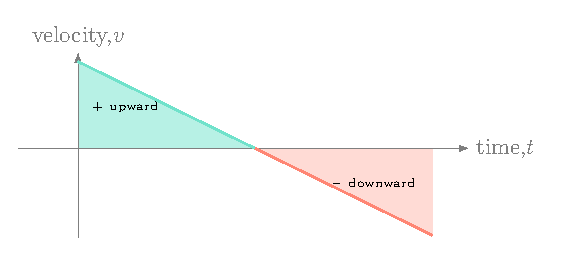
\includegraphics[width=0.8\textwidth]{verticalmotion}
\caption{竖直上抛的过程中速度大小先减小到$0$,再反向增加。加速度都是$-g$}
\end{figure}


有如下的计算公式:
\begin{table}[H]
\centering
\begin{tabular}{p{0.2\textwidth}p{0.2\textwidth}}
$v=u-gt$      & $t=\frac{v-u}{-g}$ \\ 
$h_{max}=\frac{0^2-u^2}{-2g}$ & & $s=ut-\frac{1}{2}gt^2$ 
\end{tabular}
\end{table}
当然,还有一些其他的公式,考试中可以自己独立推导。
\clearpage


\section{斜坡模型}
\label{sec:Incline Model}
斜坡模型是经典的受力分析模型之一,考察力的正交分解,以及斜坡上摩擦力和支持力的关系。如果是静止在斜坡上或者沿着斜坡匀速下滑的物块的受力分析图如下:
\begin{figure}[H]
\centering
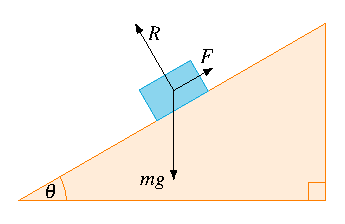
\includegraphics[width=0.8\textwidth]{inclinemodel}
\caption{再一次斜坡模型}
\end{figure}

这里需要建立以斜坡方向为$x$轴,垂直斜坡方向为$y$轴的坐标系。将重力分解到沿斜坡方向的分力与垂直斜坡方向的分力。在考虑受力平衡状态。如果恰好斜坡匀速下滑,根据牛顿第一定律可推导此时滑动摩擦力的大小就等同于重力的沿斜坡分量,支持力的大小就等同于重力垂直斜坡分量。有如下的关系
\[
	F=mg\sin \theta \hspace{2cm} R=mg\cos\theta
\]
所以再结合滑动摩擦力和支持力的关系:$f=\mu R$。即可反推处接触面之间的摩擦系数:
\[
	\mu =\tan \theta
\]

斜坡模型还有一些其他的变体和考察方式,但是基本思路都是绘制受力分析图,建立坐标系,分解重力以及其他的力,列出$x$方向上的力的关系和$y$方向上的力的关系,最后借用摩擦力和支持力的关系就可以求算加速度或者其他信息。

\begin{ExampleBox}
A particle of mass $13$ \si{\kg} is on a rough plane inclined at an angle of $\theta$ to the horizontal, where $\tan \theta =\frac{5}{12}$ . The coefficient of friction between the particle and the plane is $0.3$. A force of magnitude $T$\si{\N}, acting parallel to a line of greatest slope, moves the particle at a constant speed. Find the magnitdue of $T$\\
\makebox{}\hfill Adapted from 2019 summer qp 42 Q3
\tcblower
首先做一些准备工作,已知$\tan \theta$可以求算$\sin \theta=\frac{5}{13}$,$\cos \theta=\frac{12}{13}$\\
其次绘制受力分析图像
\begin{figure}[H]
\centering
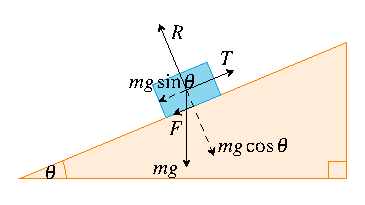
\includegraphics[width=0.5\textwidth]{2019Q3}
\caption{斜坡模型受力分析图}
\end{figure}

第三步,建立坐标系,进行两个方向上的分析。可以列出如下的相关方程:
\begin{align*}
T-mg\sin\theta-F &=0\\
R-mg\cos\theta &=0
\end{align*}

再结合滑动摩擦力与支持力的关系$F=\mu R$,最终求得$T=mg(\sin\theta+\mu \cos\theta)=86$\si{\N}
\end{ExampleBox}

\section{连接的物体之间的作用}
\label{sec:Connected Particles}
当多个物体之间通过绳子,棒子,或者直接接触进行连接。这样的物体可以当成一个完整的系统进行处理。

\subsection*{杆连接}
如果两个物体之间是通过硬质杆进行的连接,那么杆对两个物体可以产生张力,或者推力,取决于杆子的是否被拉伸或者挤压。
\begin{figure}[H]
\centering
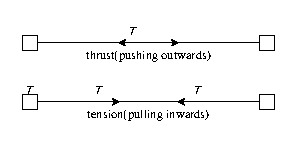
\includegraphics[width=0.8\textwidth]{rod}
\caption{杆当中既可以产生推力,也能有拉力}
\end{figure}

\subsection*{滑轮和绳链接}
对于用\emph{不可延长}的绳子连接的物体其处理方式是,绳子只能产生一样的拉力,而定滑轮则可以改变拉力的方向。所以绳子上的拉力不需要像杆一样,必须沿一条直线作用。第二点是由于绳子不可延长,因此绳的两端的运动状态必须保持大小一致
具有同样大小的速度,加速度还有位移(方向可以不同)。对两个物体分别做受力分析即可。

\begin{ExampleBox}
A smooth inclined plane of length $2.5$ \si{\m} is fixed with one end on the horizontal floor and the other end at a height of $0.7$ \si{\m} above the floor. Particles $P$ and $Q$, of masses $0.5$ \si{\kg} and $0.1$ \si{\kg} respectively, are attached to the ends of a light inextensible string which passes over a small smooth pulley fixed at the top of the plane. Particle $Q$ is held at rest on the floor vertically below the pulley. The string is taut and $P$ is at rest on the plane (see diagram). $Q$ is released and starts to move vertically upwards towards the pulley and $P$ moves down the plane.
\begin{figure}[H]
\centering
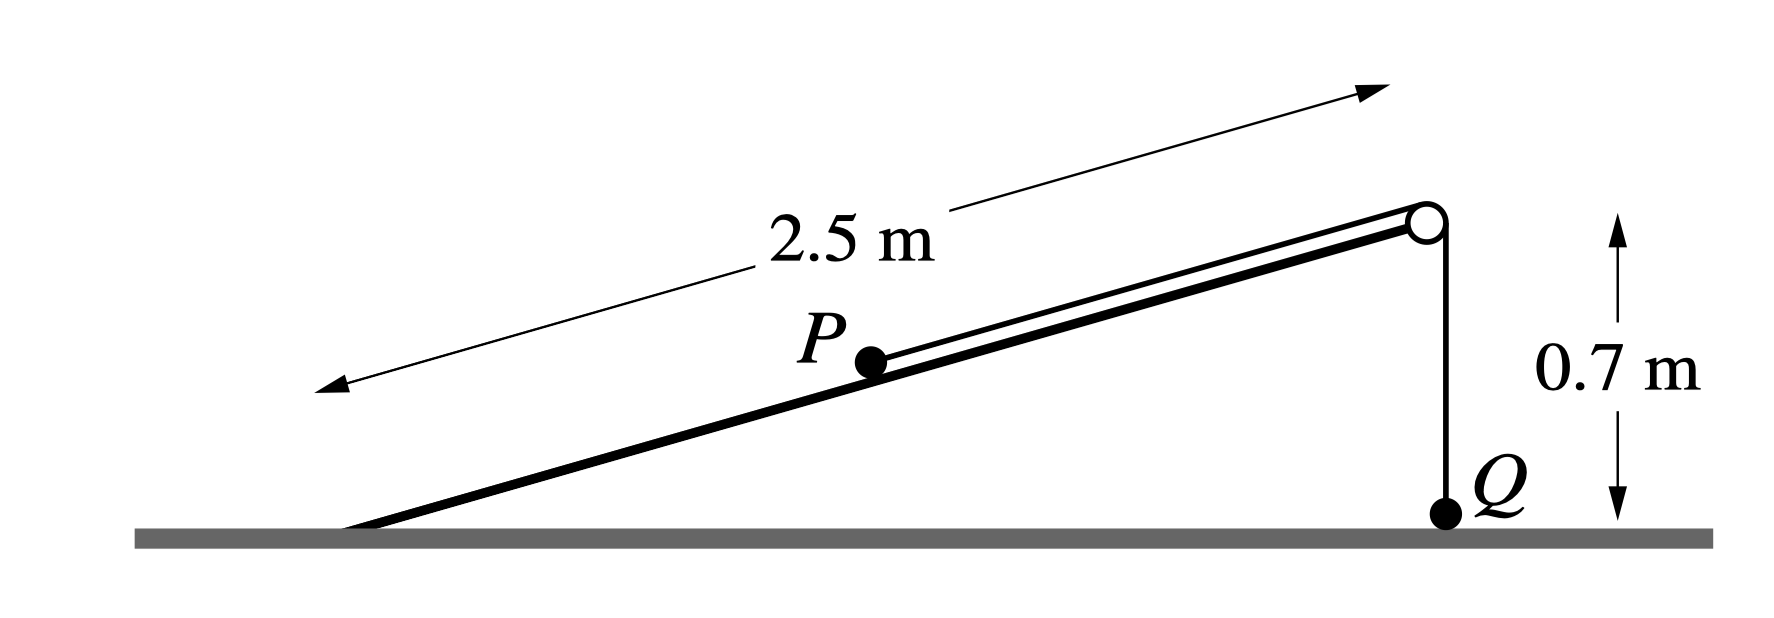
\includegraphics[width=0.5\textwidth]{inclinepulley}
\end{figure}
Find the tension in the string and the magnitude of the acceleration of the particles before $Q$ reaches the pulley.\\
\makebox{}\hfill Adapted from $2015$ winter qp $42$ $Q5$
\tcblower
对$Q$分析,受到向上的tension和向下的gravity\\
对$P$分析,受到向下的gravity,垂直于斜坡的Normal Contact Force,以及沿斜坡方向的tension(与作用在Q上的tension是一样大的,都来自与绳子)
如下图所示:
\begin{figure}[H]
\centering
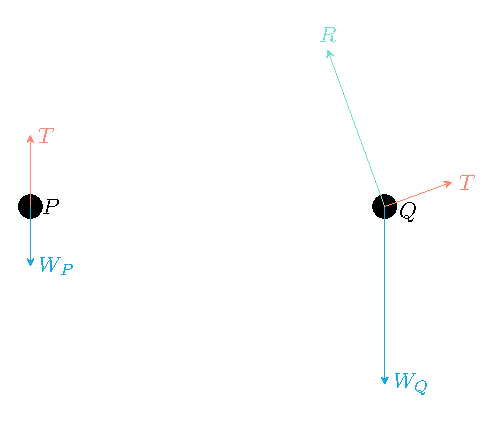
\includegraphics[width=0.8\textwidth]{fbd-system}
\end{figure}
因此可以对两个物体$P$,$Q$分别进行受力分析,列出牛顿第二定律公式来。
\begin{align*}
m_Qg\cdot \sin\theta -T &=m_Q\cdot a\\
T-m_pg &=m_P\cdot a\\
\sin\theta &=\frac{5}{27}
\end{align*}
因此可以求算出 $a=\frac{2}{3}\si{\m\per\square\s} \qquad T=\frac{16}{15} \si{\N}$
\end{ExampleBox}




